
Le vol AF 423 rejoint Bogotá à Paris en passant par Maracaïbo, La Guadeloupe, les Acores, Brest et enfin atterrit à Paris. Généralement, le temps de parcours entre Bogotá et Maracaïbo est de 1 heure et 45 minutes. Entre Maracaïbo et Brest, l'avion vole à une vitesse constante de $890 km.h^{-1}$. Puis il descend de Brest à l'aéroport Charles de Gaulle en 45 minutes. L'avion vole exclusivement en ligne droite selon les couloirs imposés par l'International Air Transport Association (IATA).


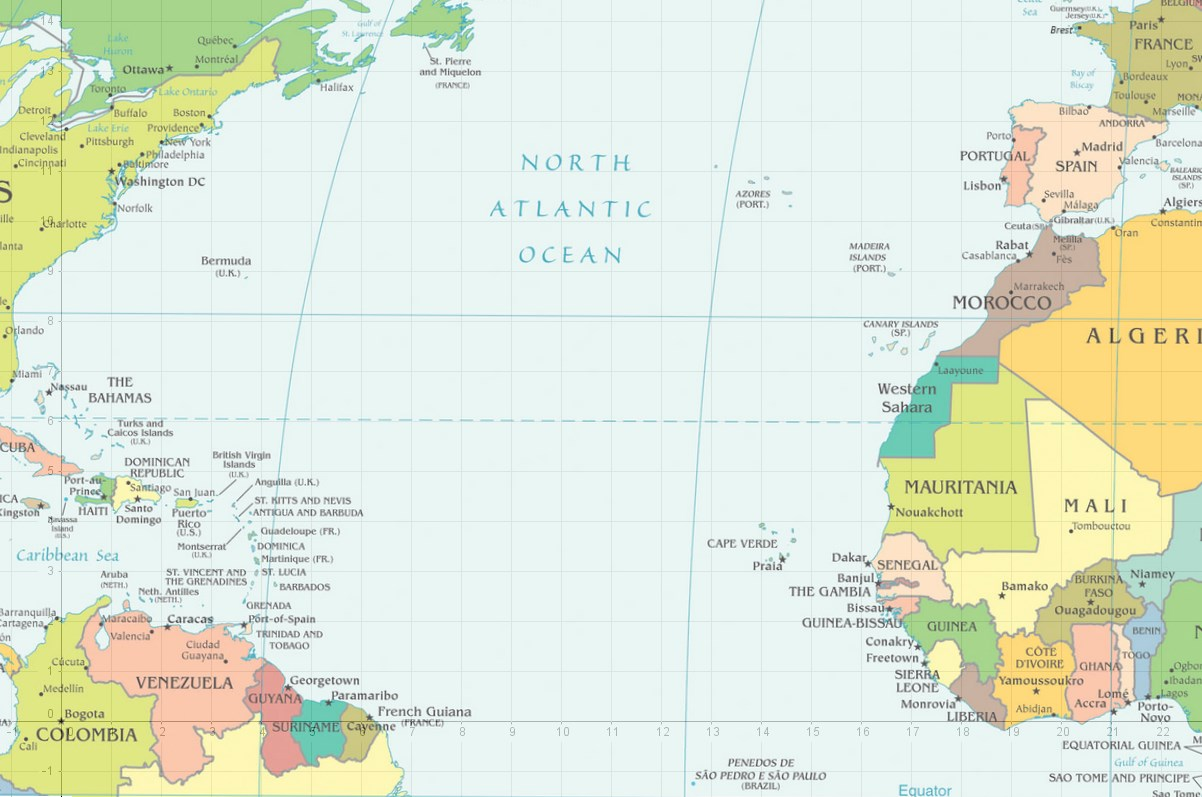
\includegraphics[scale=0.95]{ED-23.jpg} 


\begin{enumerate}
\item Déterminer le trajet que les pilotes doivent insérer dans l'ordinateur de bord de l'Airbus A340 pour parcourir le vol Bogotá-Paris
\item Déterminer le temps de vol entre Paris et Bogotá. On cherchera su internet la distance réelle Bogotá-Maracaïbo en vol direct.
\end{enumerate}